\section{PCB Design \& BOM}
\subsection{PCB Design}
The main goals of the PCB design is to create a robust, safe and user-friendly environment for the designed circuit. PCBs can be easily manufactured in bulk, therefore, they cost much less than traditional circuit building techniques. They enable the designers to make connections on multiple layers which means that they can implement fairly complex circuits on small cards which allows them to design more compact products, as size of a circuit can be critical in many applications. Furthermore, power/volume ratio which is known as Power Density is an important factor in determining the quality of the design of a power electronics circuit. 
\\There are several factors to be taken into consideration while designing a PCB such as clearances, cooling, compactness, isolation, signal and power paths. Since our circuit is a power conversion circuit, some measures must be taken to accommodate the requirements for proper operation. Switching components with significant losses are chosen as through-hole and are placed so that they can be equipped with heat sinks. Since the primary and the secondary sides of the circuit is isolated with a transformer in power path, signal path must also be isolated with an optocoupler. The isolation boundary is marked with a straight line.
\\ The PCB for our circuit is designed in KiCad environment. The schematic for the our circuit that is to be implemented on a PCB is given in Figure \ref{fig:layout}.
\begin{figure}[H]
\begin{center}
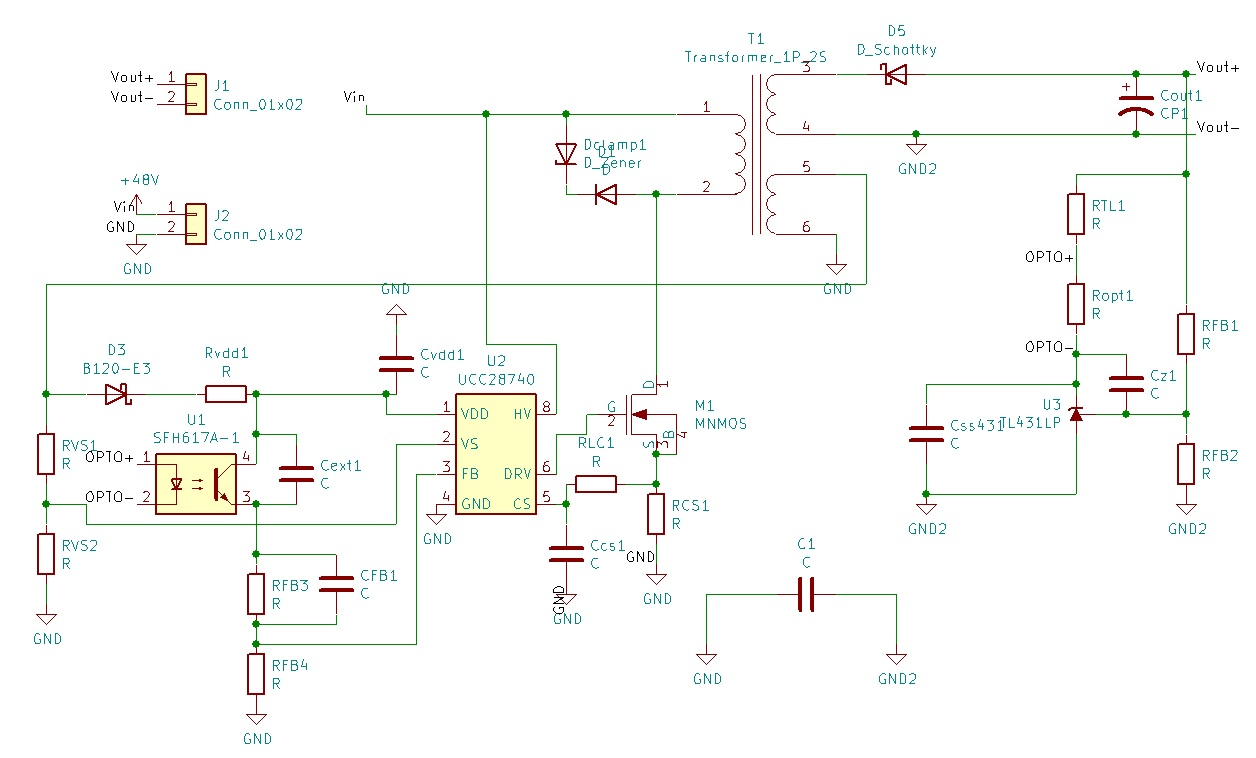
\includegraphics[width=1\textwidth]{figures/layout.jpg}
\caption{Flyback Converter Schematic}
\label{fig:layout}
\end{center}
\end{figure}
Both top and bottom layers are utilized to have a compact design. The maximum current in the circuit is 4A which is observed at the output. 4A current requires 0.24mm trace width, but to be safe, power paths consists of 1mm traces. For signal paths, 1mm and 0.5mm traces are used, depending on the density of traces in the area. To be able to connect the load and input, connections for banana plugs are placed with clear markings, as in Figure \ref{fig:bananaplug}.

\begin{figure}[H]
\begin{center}
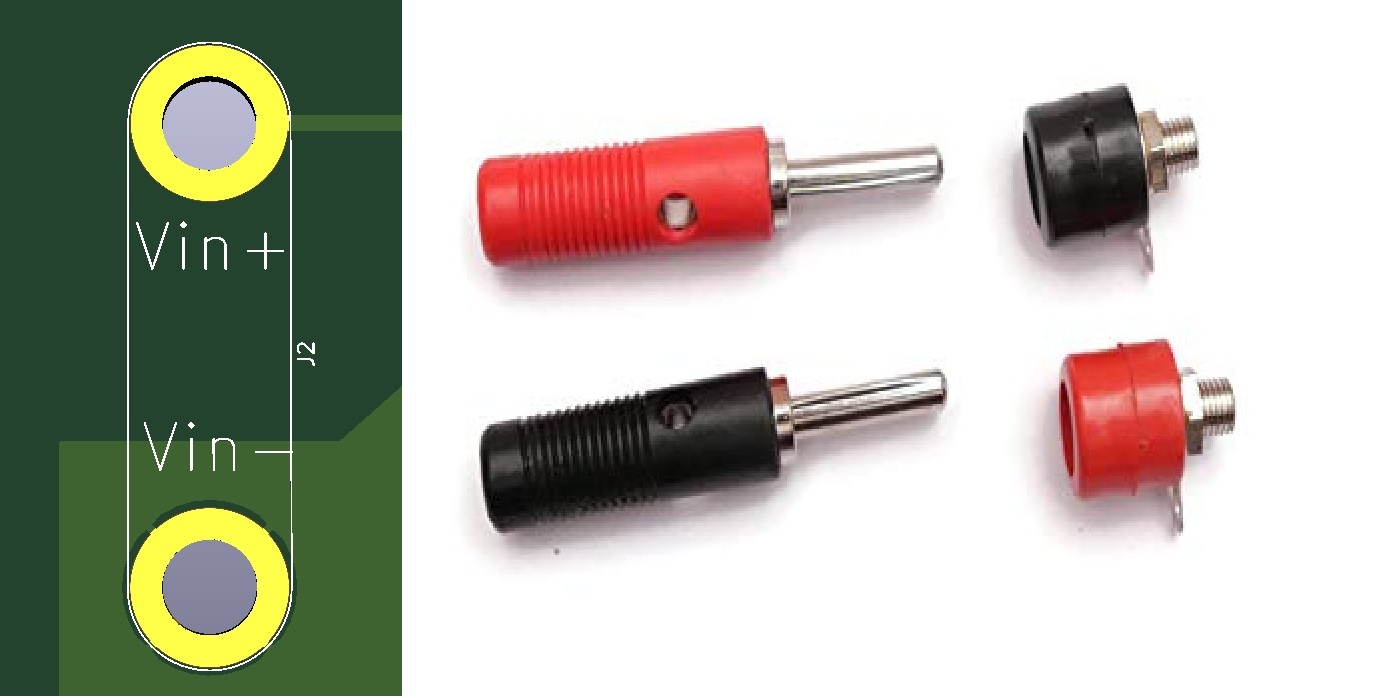
\includegraphics[width=0.8\textwidth]{figures/bananaplug.jpg}
\caption{Banana Plug and Socket(right) PCB connection (left) }
\label{fig:bananaplug}
\end{center}
\end{figure}

Not to be drastically affected by stray inductances, all the paths are optimized to be the shortest possible. This is very critical on feedback paths and MOSFET gate connections, where very sharp responses is of utmost importance. Using the guidelines given in UCC28740 datasheet, the design around the controller is carried out with extreme care as in Figure  \ref{fig:controllerdesign}.

\begin{figure}[H]
\begin{center}
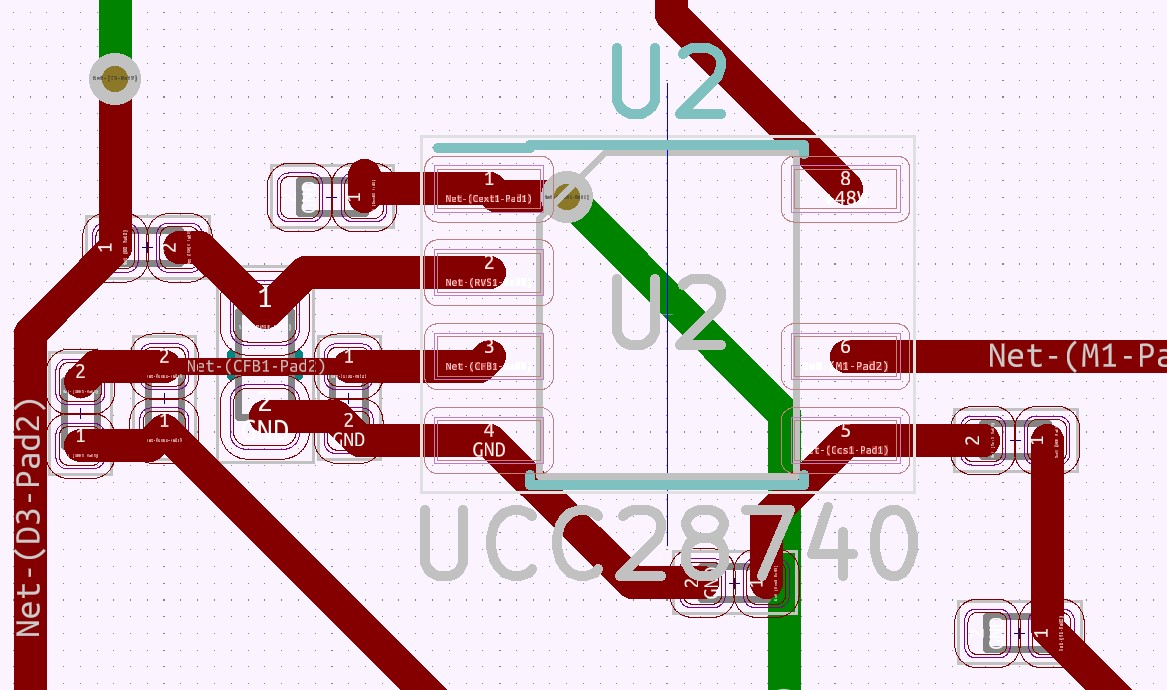
\includegraphics[width=0.8\textwidth]{figures/controllerdesign.jpg}
\caption{PCB Design Around Controller IC}
\label{fig:controllerdesign}
\end{center}
\end{figure}

2D view of the PCB is given below in Figure \ref{fig:pcb2D}. Red lines show the traces on top layer and green lines are the connections on bottom layer. The areas outlined with dashed lines are ground planes, separate for primary and secondary sides.

\begin{figure}[H]
\begin{center}
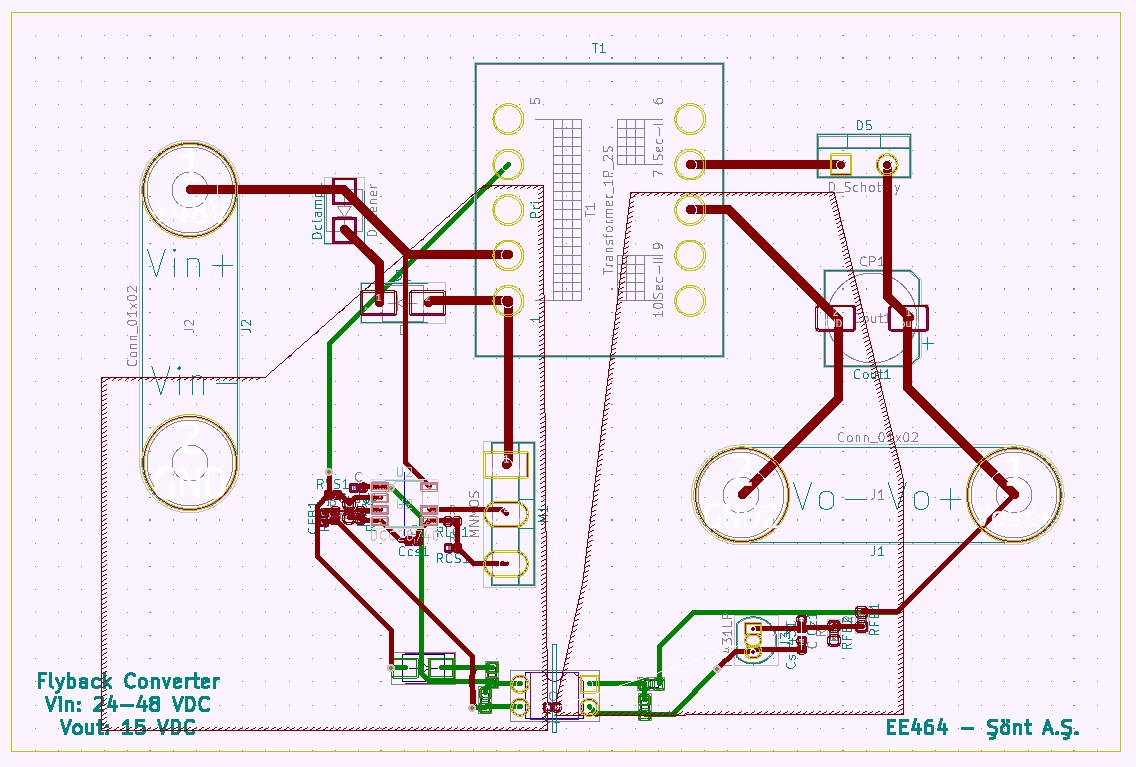
\includegraphics[width=0.8\textwidth]{figures/pcb2d.jpg}
\caption{2D View of Designed PCB}
\label{fig:pcb2D}
\end{center}
\end{figure}

Lastly, by assigning realistic footprints to each component, we have obtained the 3D view of the PCB, given in Figure \ref{fig:pcb3D}. The heat sink on the MOSFET is chosen arbitrarily, and the heat sink on the secondary diode is not shown, but necessary space is provided.

\begin{figure}[H]
\begin{minipage}{1\textwidth} 
\centering
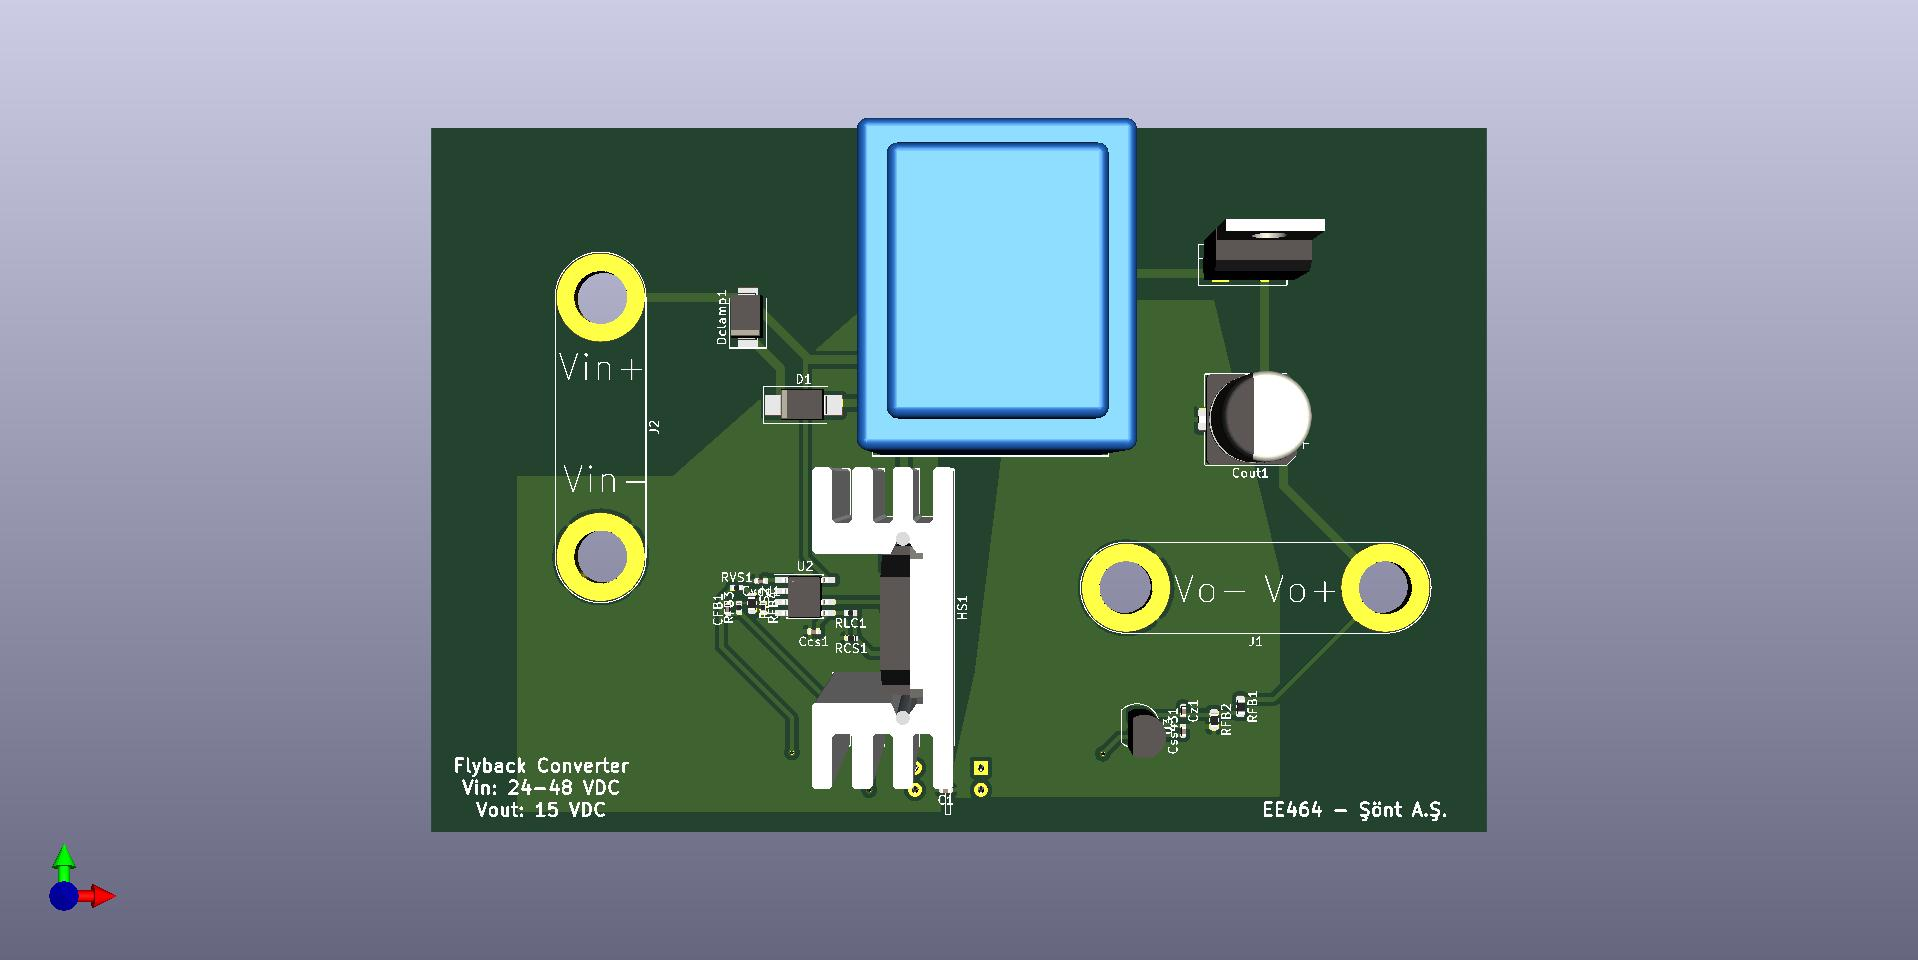
\includegraphics[width=0.8\textwidth]{figures/pcb3dtop.jpg}
\caption{Top View}
\end{minipage}    
\begin{minipage}{1\textwidth} 
\centering
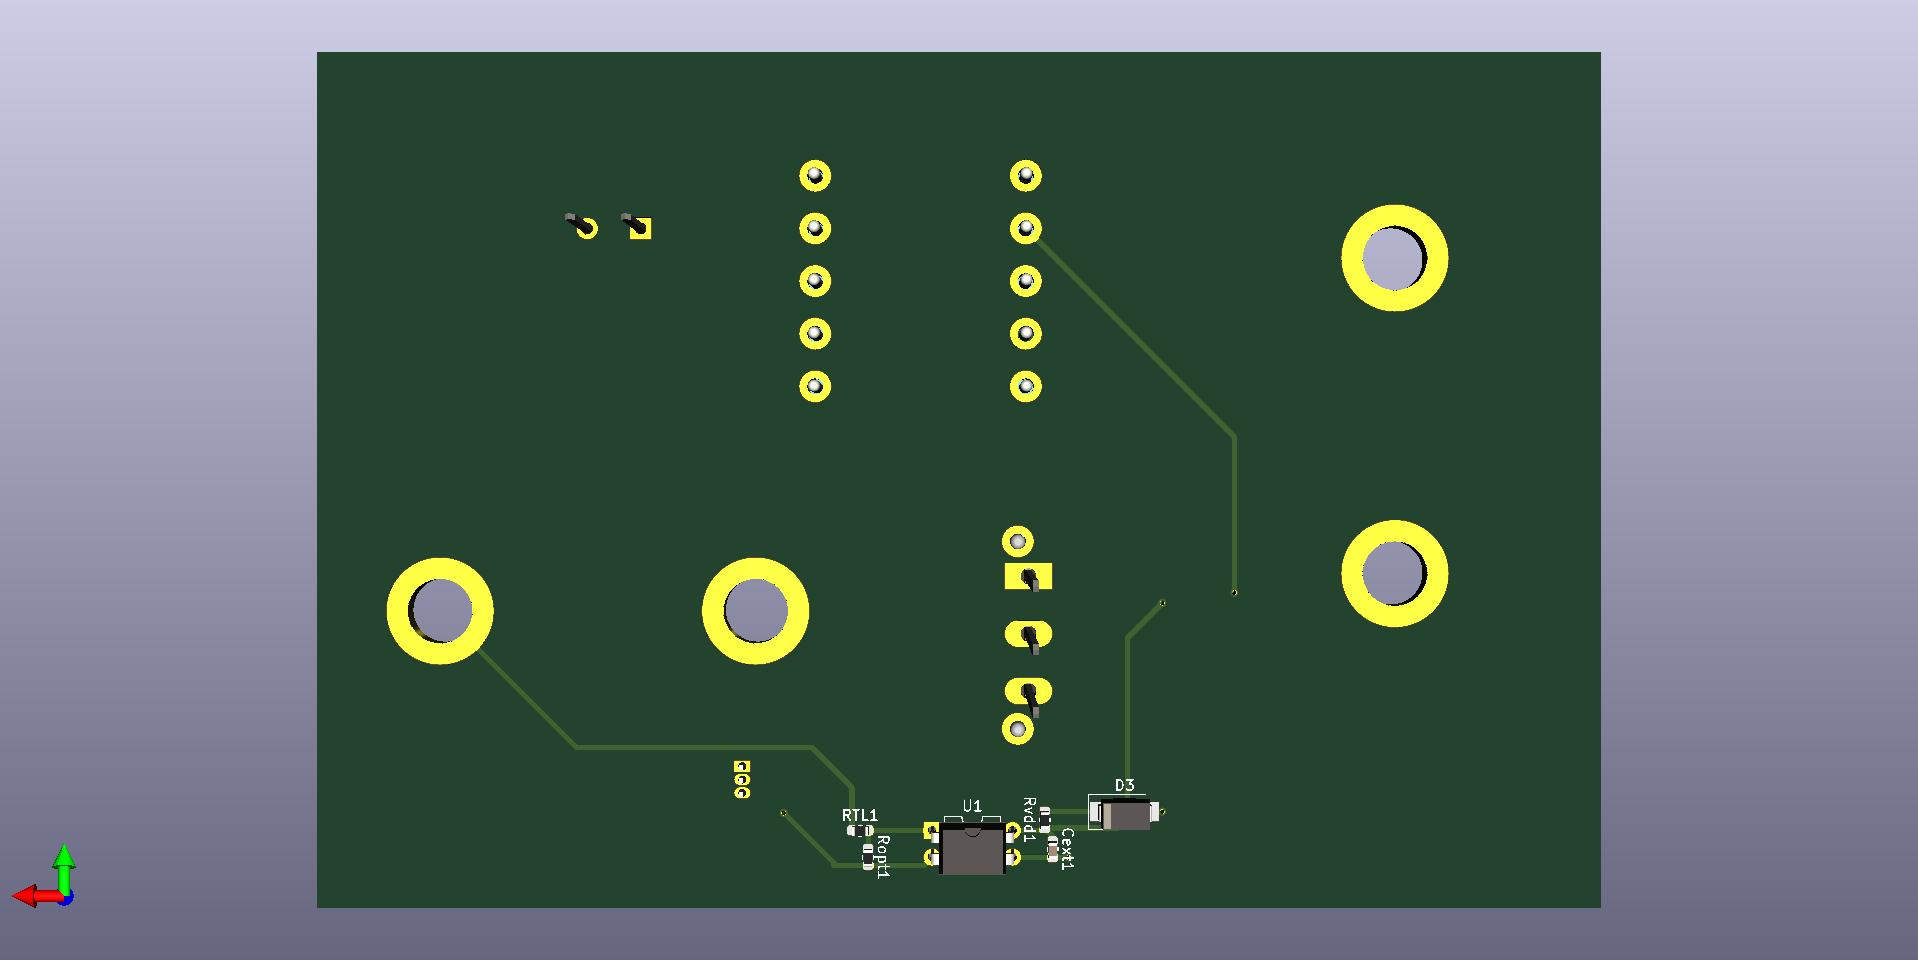
\includegraphics[width=0.8\textwidth]{figures/pcb3dbot.jpg}
\caption{Bottom View}
\end{minipage}    
\begin{minipage}{1\textwidth} 
\centering
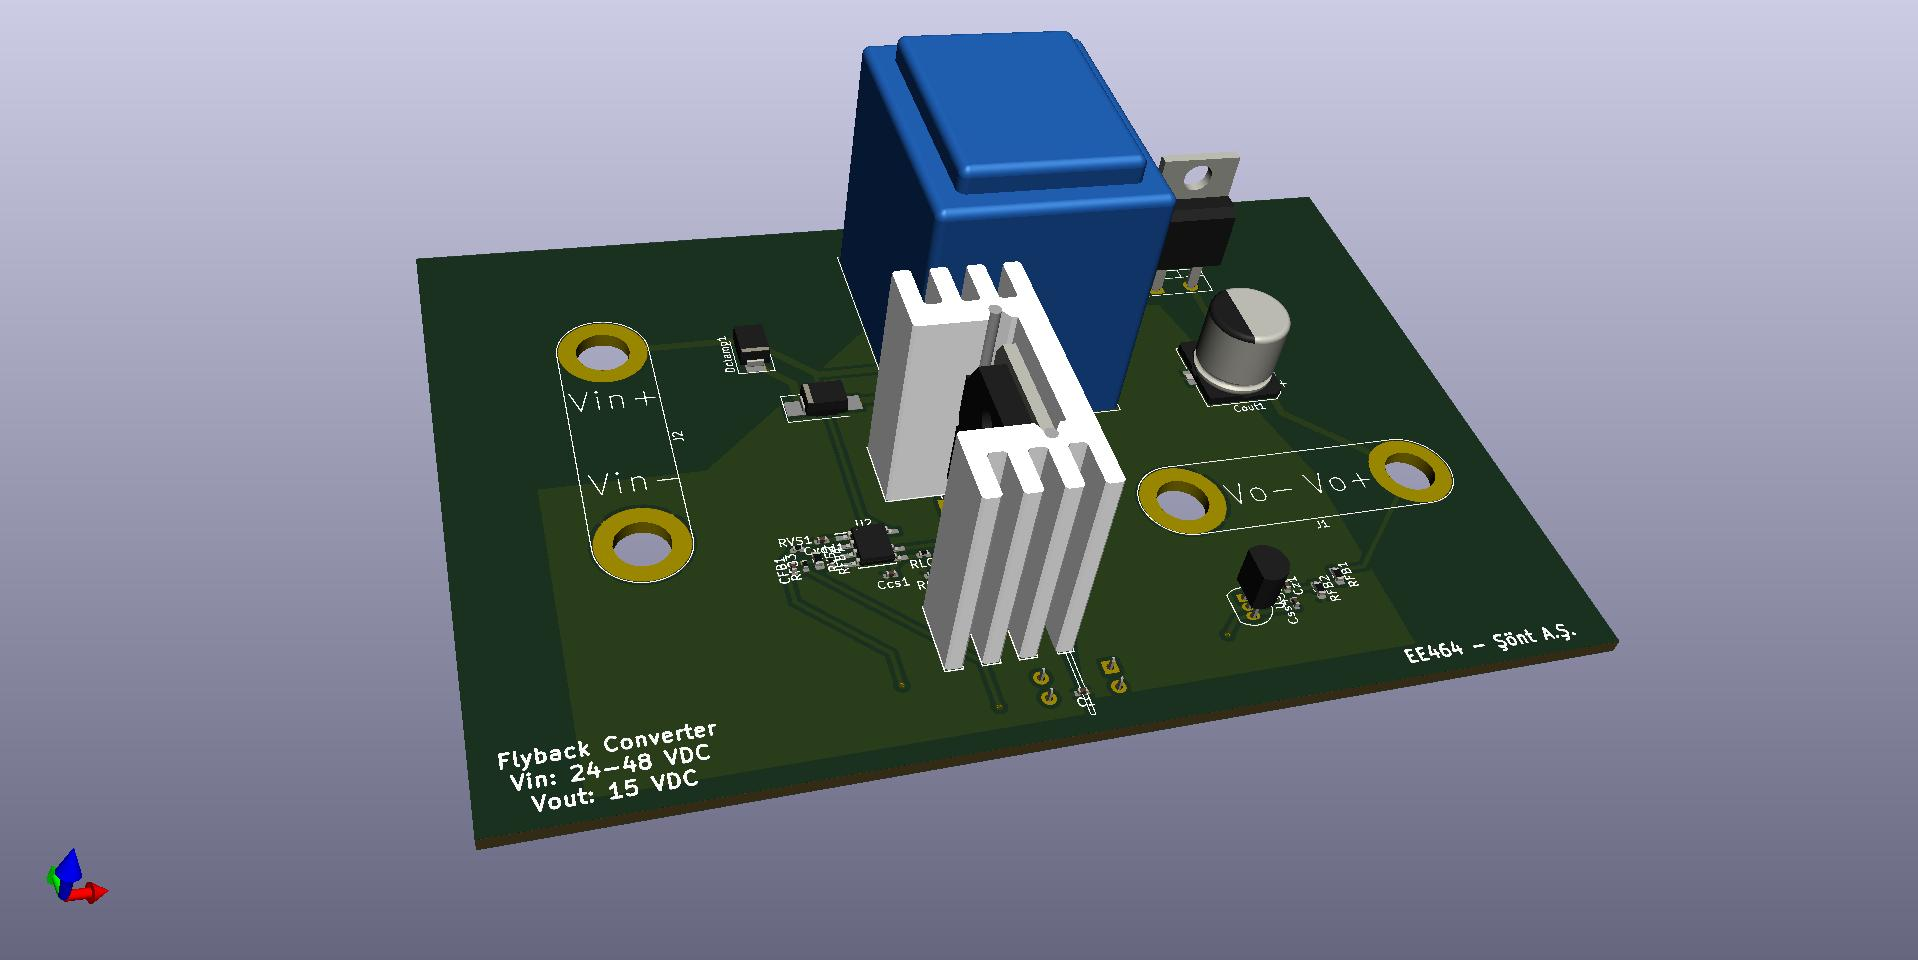
\includegraphics[width=0.8\textwidth]{figures/pcb3diso.jpg}
\caption{Isometric View}
\end{minipage}    
\caption{3D View of Designed PCB}
\label{fig:pcb3D}
\end{figure}

\subsection{Bill of Materials (BOM)}
The BOM for all the components is given in the table below. Also, we have obtained a quota from PCBWay. For 1000 boards, the PCB cost is \$ 994. Also, they asked \$387 for shipping which is estimated to arrive in 2 weeks. As a result, the total is \$1.38 for each PCB.
\begin{figure}[H]
\begin{center}
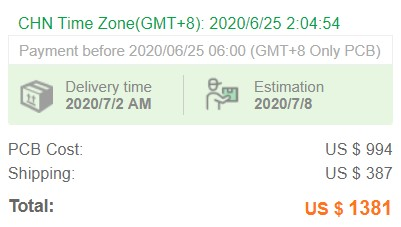
\includegraphics[width=0.8\textwidth]{figures/pcbprice.jpg}
\caption{PCB Pricing}
\label{fig:pcbprice}
\end{center}
\end{figure}
\begin{table}[H]
\resizebox{\textwidth}{!}{
\begin{tabular}{|r|l|l|l|l|l|}
\hline
Id                     & Designator                          & Supplier and ref                  & Quantity & Unit Price & Total Price \\ \hline
1                      & C1,CFB1,Cz1,Cvdd1,Css431,Ccs1,Cext1 & TDK C1608C0G1V103J080AC           & 6        & 0.04       & 0.24        \\ \hline
2                      & Transistor Heatsink                 & Assmann WSW Components, V5220L    & 1        & 0.8        & 0.8         \\ \hline
3                      & Diode Heatsink                      & CUI Devices, HSS-B20-NP-01        & 1        & 0.2        & 0.2         \\ \hline
4                      & D5                                  & ON Semi, MBR10100G                & 1        & 0.85       & 0.85        \\ \hline
5                      & RVS1,RLC1,RFB3,RFB4,RCS1            & Yageo,	RC0402FR                   & 5        & 0.001      & 0.005       \\ \hline
6                      & TL431LP                             & Texas Instruments                 & 1        & 0.124      & 0.124       \\ \hline
7                      & Cout1                               & Panasonic,EEE1HA211P              & 1        & 0.62       & 0.62        \\ \hline
8                      & Dclamp1                             & Vishay, MSP3V3                    & 1        & 0.08       & 0.08        \\ \hline
9                      & D1                                  & ON Semi, BAT54HT1G                & 1        & 0.041      & 0.041       \\ \hline
10                     & J1,J2 (Banana\_Jack\_2Pin)          & Cinch Connectivity                & 4        & 0.6        & 2.4         \\ \hline
11                     & Rvdd1,RTL1,Ropt1,RFB2,RFB1,RVS2     & Yageo, RC0603JR                   & 6        & 0.002      & 0.012       \\ \hline
12                     & D3                                  & Vishay, B120-E3                   & 1        & 0.08       & 0.08        \\ \hline
13                     & U2                                  & Texas Instruments, UCC28740DR     & 1        & 0.46       & 0.46        \\ \hline
14                     & Transformer Core                    & Magnetics, 00K2510E090            & 1        & 4.17       & 4.17        \\ \hline
15                     & Transformer Bobbin                  & Ferroxcube, CSH-EP13-1S-10P-T     & 1        & 0.25       & 0.25        \\ \hline
16                     & U1                                  & Isocom, SFH617A-2X                & 1        & 0.59       & 0.59        \\ \hline
17                     & M1                                  & STMicroelectronics,  STP17NK40ZFP & 1        & 3.3        & 3.3         \\ \hline
18                     & PCB                                 & PCBWay                            & 1        & 1.38        & 1.38         \\ \hline
\multicolumn{1}{|l|}{} &                                     &                                   &          &            & 15.602      \\ \hline
\end{tabular}}
\caption{Bill of Materials}
\end{table}

Material cost for or Flyback Converter is estimated to be \$15.6.

\newpage